\documentclass{beamer}
\let\vec\mathbf
\mode<presentation>
\usepackage{amsmath}
\usepackage{amssymb}
%\usepackage{advdate}
\usepackage{adjustbox}
%\usepackage{subcaption}
\usepackage{enumitem}
\usepackage{multicol}
\usepackage{mathtools}
\usepackage{listings}
\usepackage{url}
\usetheme{Boadilla}
\usecolortheme{lily}
\setbeamertemplate{footline}
{
  \leavevmode%
  \hbox{%
  \begin{beamercolorbox}[wd=\paperwidth,ht=2.25ex,dp=1ex,right]{author in head/foot}%
    \insertframenumber{} / \inserttotalframenumber\hspace*{2ex} 
  \end{beamercolorbox}}%
  \vskip0pt%
}
\setbeamertemplate{navigation symbols}{}
\providecommand{\nCr}[2]{\,^{#1}C_{#2}} % nCr
\providecommand{\nPr}[2]{\,^{#1}P_{#2}} % nPr
\providecommand{\mbf}{\mathbf}
\providecommand{\pr}[1]{\ensuremath{\Pr\left(#1\right)}}
\providecommand{\qfunc}[1]{\ensuremath{Q\left(#1\right)}}
\providecommand{\sbrak}[1]{\ensuremath{{}\left[#1\right]}}
\providecommand{\lsbrak}[1]{\ensuremath{{}\left[#1\right.}}
\providecommand{\rsbrak}[1]{\ensuremath{{}\left.#1\right]}}
\providecommand{\brak}[1]{\ensuremath{\left(#1\right)}}
\providecommand{\lbrak}[1]{\ensuremath{\left(#1\right.}}
\providecommand{\rbrak}[1]{\ensuremath{\left.#1\right)}}
\providecommand{\cbrak}[1]{\ensuremath{\left\{#1\right\}}}
\providecommand{\lcbrak}[1]{\ensuremath{\left\{#1\right.}}
\providecommand{\rcbrak}[1]{\ensuremath{\left.#1\right\}}}
\theoremstyle{remark}
\newtheorem{rem}{Remark}
\newcommand{\sgn}{\mathop{\mathrm{sgn}}}

\providecommand{\res}[1]{\Res\displaylimits_{#1}} 
\providecommand{\norm}[1]{\lVert#1\rVert}
\providecommand{\mtx}[1]{\mathbf{#1}}

\providecommand{\fourier}{\overset{\mathcal{F}}{ \rightleftharpoons}}
%\providecommand{\hilbert}{\overset{\mathcal{H}}{ \rightleftharpoons}}
\providecommand{\system}{\overset{\mathcal{H}}{ \longleftrightarrow}}
 %\newcommand{\solution}[2]{\textbf{Solution:}{#1}}
%\newcommand{\solution}{\noindent \textbf{Solution: }}
\providecommand{\dec}[2]{\ensuremath{\overset{#1}{\underset{#2}{\gtrless}}}}
\newcommand{\myvec}[1]{\ensuremath{\begin{pmatrix}#1\end{pmatrix}}}

\title{Matrices in Geometry - 10.7.84}
\author{EE25BTECH11035 Kushal B N}
\date{}

\begin{document}

\maketitle

\section{Problem Statement}
\begin{frame}
\frametitle{Problem Statement}
Let $2x^2 + y^2 - 3xy = 0$ be the equation of pair of tangents drawn from the origin $\vec{O}$ to a circle of radius 3 with the centre in the first quadrant. If $\vec{A}$ is one of the points of contact, find the length of \textit{OA}.
\hfill (JEE 2001)
\end{frame}

\section{Solution}
\begin{frame}{Solution}
Given,
The equation of pair of tangents
\begin{equation}
    y^2 - 3xy + 2x^2 = 0
\end{equation}
Radius $r = 3$

Factorising the given equation of pair of tangents
\begin{equation}
    (y-x)(y-2x) = 0
\end{equation}

The direction vectors of the two tangent lines from the origin 
\begin{equation}
    \vec{m}_1 = \myvec{1\\1}
\end{equation}
\begin{equation}
    \vec{m}_2 = \myvec{1\\2}
\end{equation}
\end{frame}

\begin{frame}{Solution}
Now, let $2\phi$ be the angle between the two tangent lines.
\begin{equation}
    \vec{m}_1^{\top}\vec{m}_2 = \myvec{1&1}\myvec{1\\2} = 3
\end{equation}

\begin{equation}
    \norm{\vec{m}_1} = \sqrt{\vec{m}_1^{\top}\vec{m}_1} = \sqrt{2}
\end{equation}

\begin{equation}
    \norm{\vec{m}_2} = \sqrt{\vec{m}_2^{\top}\vec{m}_2} = \sqrt{5}
\end{equation}

\begin{equation}
    \cos{2\phi} = \frac{\vec{m}_1^{\top}\vec{m}_2}{\norm{\vec{m}_1}\norm{\vec{m}_2}} = \frac{3}{\sqrt{2}\sqrt{5}} = \frac{3}{\sqrt{10}}
\end{equation}

\begin{equation}
    \implies \tan{2\phi} = \frac{\sqrt{1 - \cos^2{2\phi}}}{\cos{2\phi}} = \frac{1/\sqrt{10}}{3\sqrt{10}} = \frac{1}{3}
\end{equation}

\end{frame}

\begin{frame}{Solution}
Let the centre of the circle be $\vec{C}$, so that in the right-angled triangle $\Delta OAC$, we have (as $AC = r = 3$)
\begin{equation}
    \tan{\phi} = \frac{AC}{OA} = \frac{3}{OA}
\end{equation}

\begin{equation}
    \tan{2\phi} = \frac{2\tan{\phi}}{1 - \tan^2{\phi}}
\end{equation}
Let $t = \tan{\phi}$

\begin{equation}
    \frac{1}{3} = \frac{2t}{1 - t^2}
\end{equation}

\begin{equation}
    \implies t^2 + 6t -1 = 0
\end{equation}
\end{frame}

\begin{frame}{Solution}
    Solving the above quadratic equation using the quadractic formula, we get

\begin{equation}
    t = -3 \pm \sqrt{10}
\end{equation}
Now, the angle being acute implies that $\tan{\phi} > 0$, so
\begin{equation}
    \tan{\phi} = \sqrt{10} - 3
\end{equation}

\begin{equation}
    \implies OA = \frac{3}{\tan{\phi}} = \frac{3}{\sqrt{10} - 3}
\end{equation}

Rationalising the denominator, we get
\begin{equation}
    \fbox{$OA = 9 + 3\sqrt{10}$}
\end{equation}
\end{frame}

\section{Final Answer}
\begin{frame}{Final Answer}
$\therefore$ The length of $OA$ is equal to $9 + 3\sqrt{10}$ units.
\begin{figure}[H]
    \centering
    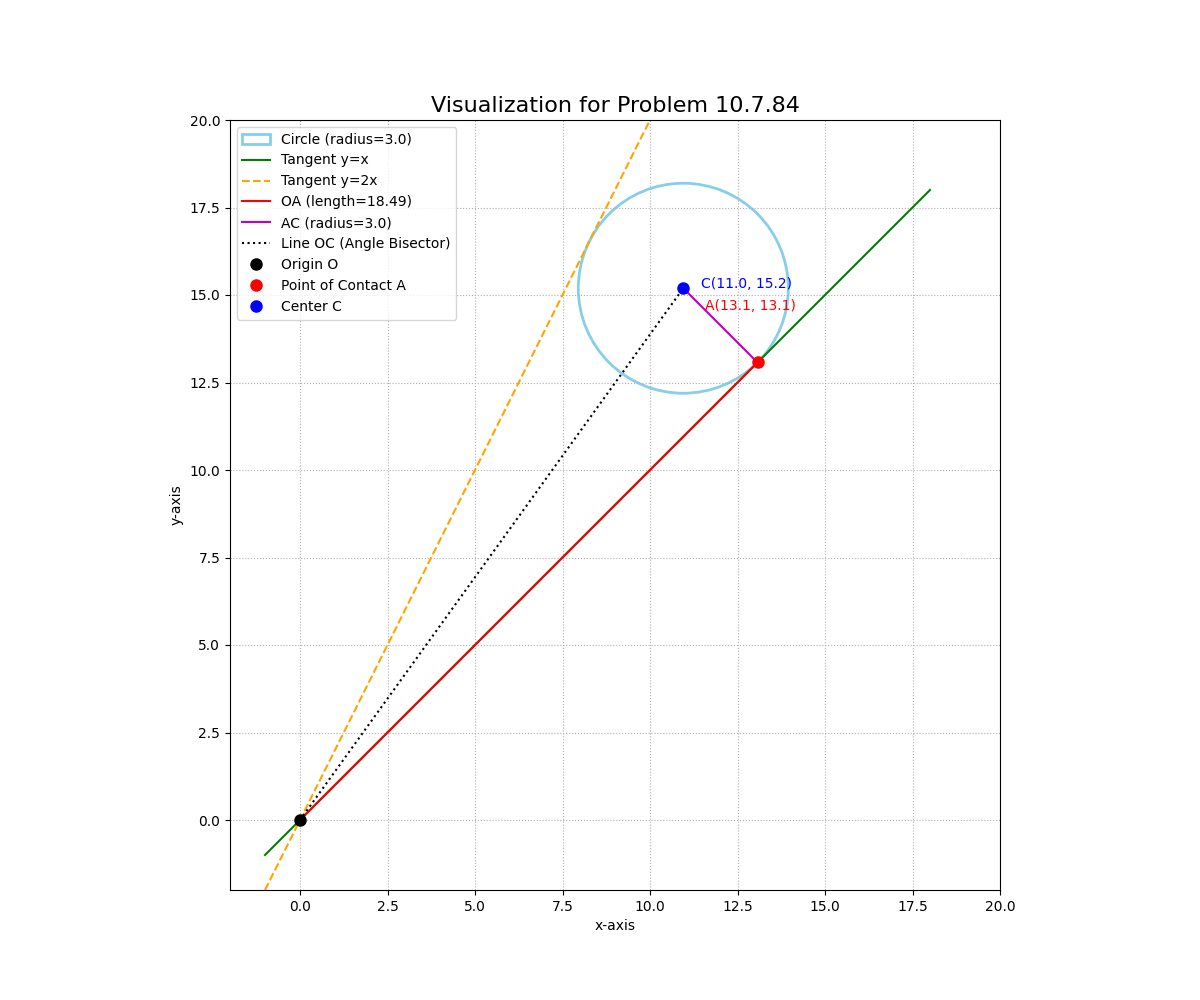
\includegraphics[width=0.60\columnwidth]{figs/2.png}
    \caption{Plot for 10.7.84}
\end{figure}
\end{frame}
\end{document}
